\section{Software Quality}
\label{sec:lit-review:software-quality}

\epigraph{Quality... you know what it is, yet you don't know what it is.}{Robert Pirsig, 1974 \citep{Pirsig:1974vs}}

\noindent
The philosophical viewpoint of `quality' remains highly debated and there are multiple facets to perceive this complex concept \citep{Garvin:1984vf}. Transcendentally, a viewpoint like that of \citeauthor{Pirsig:1974vs}'s quote above shows that quality is not tangible but still recognisable; it's hard to explicitly define but you know when it's missing. Pragmatically, the \citeauthor{ISO8402:1986} provides a breakdown of seven universally-applicable principles that defines quality for organisations, developers, customers and training providers \citep{ISO9000:2015}. More pertinently, though, the since withdrawn \citeyear{ISO8402:1986} standard for quality was simply ``the totality of characteristics of an entity that bear on its ability to satisfy stated or implied needs'' \citep{ISO8402:1986}.

Using this sentence, what characteristics exist for non-deterministic systems like that of a computer vision \gls{cis}? How do we know when the system has satisfied its `stated or implied needs' when the system can only give us uncertain probabilities in its outputs? Such answers can be derived from related definitions---such as `conformance to specification or requirements' \citep{Gilmore:1974um,Crosby:1979uy}, `meeting or exceeding customer expectation' \citep{Parasuraman:1988wh}, or `fitness for use' \citep{Juran:1988tg}---but these then still depend on the solution description or requirements specification, and thus the same questions still apply.

\textit{Software} quality is somewhat more concrete. \citet{Pressman:2005vf} adapted the manufacturing-oriented view of quality from \citep{Bessin:2004vc} and phrased software quality under three core pillars:

\begin{itemize}
  \item \textbf{effective software processes}, where the infrastructure that supports the creation of quality software needs is effective, i.e., poor checks and balances, poor change management and a lack of technical reviews (all that lie in the \textit{process} of building software, rather than the software itself) will inevitably lead to a poor quality product and vice-versa;
  \item \textbf{building useful software}, where quality software has fully satisfied the end-goals and requirements of all stakeholders in the software (be it explicit or implicit requirements) \textit{in addition to} delivering these requirements in reliable and error-free ways; and lastly
  \item \textbf{adding value to both the producer and user}, where quality software provides a tangible value to the community or organisation using it to expedite a business process (increasing profitability or availability of information) \textit{and} provides value to the software producers creating it whereby  customer support, maintenance effort, and bug fixes are all reduced in production.
\end{itemize}

In the context of a non-deterministic \gls{cis}, however, are any of the above actually guaranteed? Given that the core of a system built using on top of a \gls{cis} is fully dependent on the \textit{probability} that an outcome is true, what assurances must be put in place to provide developers with the checks and balances needed to ensure that their software is built with quality? For this answer, we re-explore the concept of \glsx{vv}.

\subsection{Validation and Verification}
\label{ssec:lit-review:software-quality:v-and-v}

In his works on software reliability \citep{Pham:2000ua,Pham:2006gy}, \citeauthor{Pham:2000ua} recounts the tale of a high-school student who sat a standardised test send out to 350,0000 students \citep{Tabor:1997tw}. In the multiple-choice mathematical problem, the examiners used an algebraic equation using the letter $a$ and intended that students \textit{assume} that $a$ was positive. The student, assuming that $a$ could also be negative, answered the `incorrect' choice of D instead of the `correct' choice of C. After contacting the examiners to point out the flaw that \textit{both} answers were indeed correct, up to 45,000 students had their scores retrospectively boosted by up to 30 points. However, by the time the score alteration was made, students had already been admitted to a university (or not), and some suggested that a 10 point difference in score can alter the outcome of a university admittance or scholarship. The outcomes of a student's higher education were, thereby, affected by this one oversight in quality assessment.

So, it seems, the examiners had mislead students to answer `incorrectly', leading to an poor question being written, and poor process standards to check if their `correct' answers were indeed 100\% correct. In the words of \citet{Boehm:1981ua}, the examiners ``didn't build the right product'' (exam) to effectively examine students, nor did they ``build the product right'' by failing to ensure quality standards were in their processes. 

This story analogously describes the issues with the cost of quality \citep{Boehm:2005vj} and the importance of \gls{vv}: just as the poorly written exam question had such a high toll the 45,000 unlucky students, so does poorly written software in production. As summarised by \citet{Pressman:2005vf}, data sourced from \citet{Cigital:2003tl} in a large-scale application showed that the difference in cost to fix a bug in development versus system testing is \$6,159 per error. In safety-critical systems, such as self-driving cars or clinical decision support systems, this cost skyrockets due to the extreme discipline needed to minimise error \citep{Tassey:2002vu}.

Formally, we refer to the IEEE Standard Glossary of Software Engineering Terminology~\citep{IEEE:1990wp} for to define \gls{vv}:

\begin{description}[font=\itshape,style=multiline,leftmargin=3cm]
  \item[verification] The process of evaluating a system or component to determine whether the products of a given development phase satisfy the conditions imposed at the start of that phase.
  \item[validation] The process of evaluating a system or component during or at the end of the development process to determine whether it satisfies specified requirements. 
\end{description} 

\noindent
Thus, in the context of a \gls{cis}, we have two perspectives on \gls{vv}: that of the \gls{api} provider and consumer (\cref{fig:lit-review:software-quality:v-and-v:leakage}).

The verification process of \gls{api} providers `leak' out to the context of the developer's project dependent on the \gls{cis}. Poor verification in the \textit{internal quality} of the \gls{cis} will entail poor process standards, such as poor definitions and terminology used, support tooling and description of documentations \citep{Sommerville:2011uc}. Though it is commonplace for providers to have a `ship-first-fix-later' mentality of `good-enough' software \citep{Venners:2003vw}, the consequence of doing so leads to consumers absorbing the cost. Thus \gls{api} providers must ensure that their verification strategies are rigorous enough for the consumers in the myriad contexts they wish to use it in; for a computer vision \gls{cis}, what might this entail? Which assurances are given to the consumers, and how is that information communicated? To verify if the service is working correctly, does that mean that we need to deploy the system first to get a wider range of data given the stochastic nature of the black box?

Likewise, the validation perspective comes from that of the consumer. While the former perspective is of creation, this perspective comes from end-user (developer) expectation. As described in \cref{ch:introduction}, a developer calls the \gls{cis} component using an API endpoint. Again, the mindset problem arises; does the developer know what to expect in the output? What are their expectations for their specific context? In the area of non-deterministic systems of probabilistic output, can the developer be assured that what they enter in a testing phase outcome the same result when in production?

\begin{figure}[hbt]
  \centering
  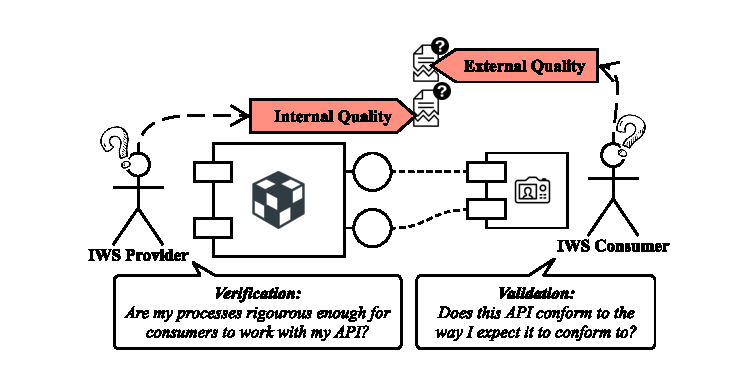
\includegraphics[width=0.8\linewidth]{leakage}
  \caption[Leakage of internal and external quality in CISs]{The `leakage' of internal quality into the API consumer's product and external quality imposing on the API provider.}
  \label{fig:lit-review:software-quality:v-and-v:leakage}
\end{figure}

Therefore, just as the high-school student's test answers in the example we opened with are both correct and incorrect at the same time, so do \glspl{cis} in returning a probabilistic result: no result is certain. While \gls{vv} has been investigated in the area of mathematical and earth sciences for numerical probabilistic models and natural systems \citep{Oreskes:1994gn,Rutten:2004a}, from the software engineering literature, little work has been achieved to look at the surrounding area of probabilistic systems hidden behind \gls{api} calls. 

Now that a developer is using  a probabilistic system behind a deterministic \gls{api} call, what does it mean in the context of \gls{vv}? Do the current verification approaches and tools do suffice, and if not, how do we fix it? From a validation perspective of \gls{ml} and end-users, after a model is trained and an inference is given and if the output data point is clearly incorrect, how will end users report a defect in the system? Compared to deterministic systems where such tooling as defect reporting forms are filled out (i.e., given input data in a given situation and the output data was X), how can we achieve similar outputs when the system is not non-deterministic? A key problem with the probabilistic mindset is that once a model is `fixed' by retraining it, while one data-point may be fixed, others may now have been effected, thereby not ensuring 100\% validation. Thus, due to the unpredicatable and blurry nature of probabilistic systems, \gls{vv} must be re-thought out extensively.

\subsection{Quality Attributes and Models}

As we follow on from \gls{vv}, we investigate similar approaches to the quality models that are used to try and capture some of the internal and external quality attributes via measurable metrics. There is no `one' definition of quality and different perspectives on the issue has lead to different users placing varying value on disparate attributes.

Quality attribute assessment models are an early concept in software engineering, and systematically evaluating software quality appears as early as \citeyear{Rubey:1968fg} \citep{Rubey:1968fg}. This study introduced `attributes' as a ``prose expression of the particular quality of desired software'' (as worded by \citet{Boehm:1978vv}) and `metrics' as mathematical parameters on a scale of 0 to 100. 
Early attempts to categorise wider factors under a framework was proposed by \citeauthor*{McCall:1977uy} in the late 1970s~\citep{McCall:1977wm,Cavano:1978gz}. This model described quality from the three perspectives of product revision (\textit{how can we keep the system operational?}), transition (\textit{how can we migrate the system as needed?}) and operation (\textit{how effective is the system at achieving its tasks?}) (\cref{fig:lit-review:software-quality:quality-models:development:mccall}). The model also introduced 11 attributes alongside numerous direct and indirect measures to help quantify quality.
This model was further developed by \citet{Boehm:1978vv} who independently developed a model resembling McCall's, starting from an initial set of 11 software characteristics similar to that of McCall's but then diving deeper by defining candidate measurements of Fortran code to such characteristics, taking shape in a tree-like structure as in \cref{fig:lit-review:software-quality:quality-models:development:boehm}. 
In the mid-1990s, Dromey's interpretation \citep{Dromey:1995wy} defined a set of quality-carrying properties with structural forms associated to specific programming languages and conventions (\cref{fig:lit-review:software-quality:quality-models:development:dromey}). The model also supported quality defect identification and proposed an improved auditing method to automate defect detection for code editors in IDEs. 
As the need for quality models became prevalent, the \citeauthor{ISO9126:1999} standardised software quality under ISO-9126 \citep{ISO9126:1999} (the Software Product Evaluation Characteristics, \cref{fig:lit-review:software-quality:quality-models:development:iso}), which has since recently been revised to ISO-25010 with the introduction of the \gls{SQuaRE} model \citep{ISO25010:2011}.
An extensive review on the development of quality models in software engineering is given in \citep{AlQutaish:2010vua}.

\begin{figure}[htp]
  \centering
  \begin{subfigure}[b]{0.49\linewidth}
    \centering
    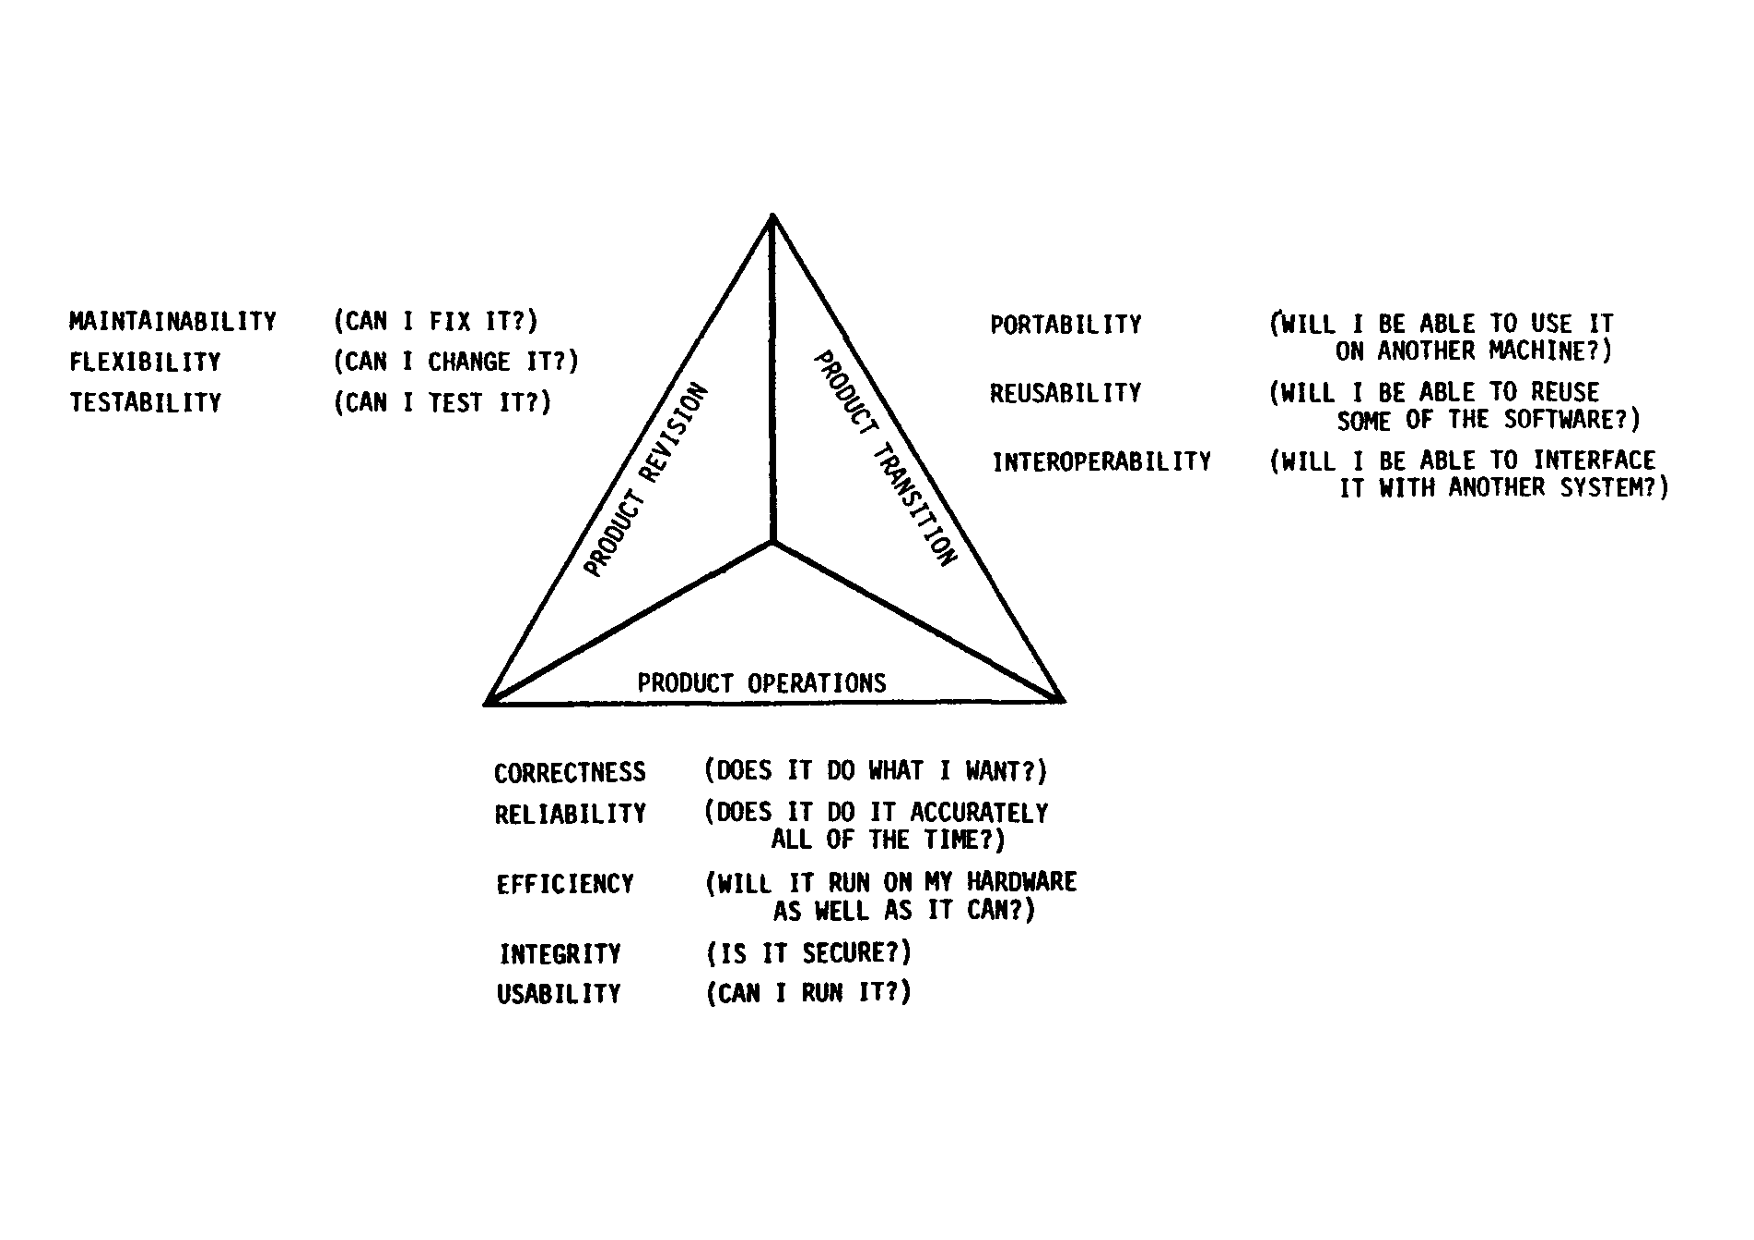
\includegraphics[width=\linewidth]{mcalls-quality-software-factors}
    \caption{McCall's Quality Software Factors (\citeyear{McCall:1977wm}) \citep{McCall:1977wm}.}
    \label{fig:lit-review:software-quality:quality-models:development:mccall}
  \end{subfigure}
  ~
  \begin{subfigure}[b]{0.49\linewidth}
    \centering
    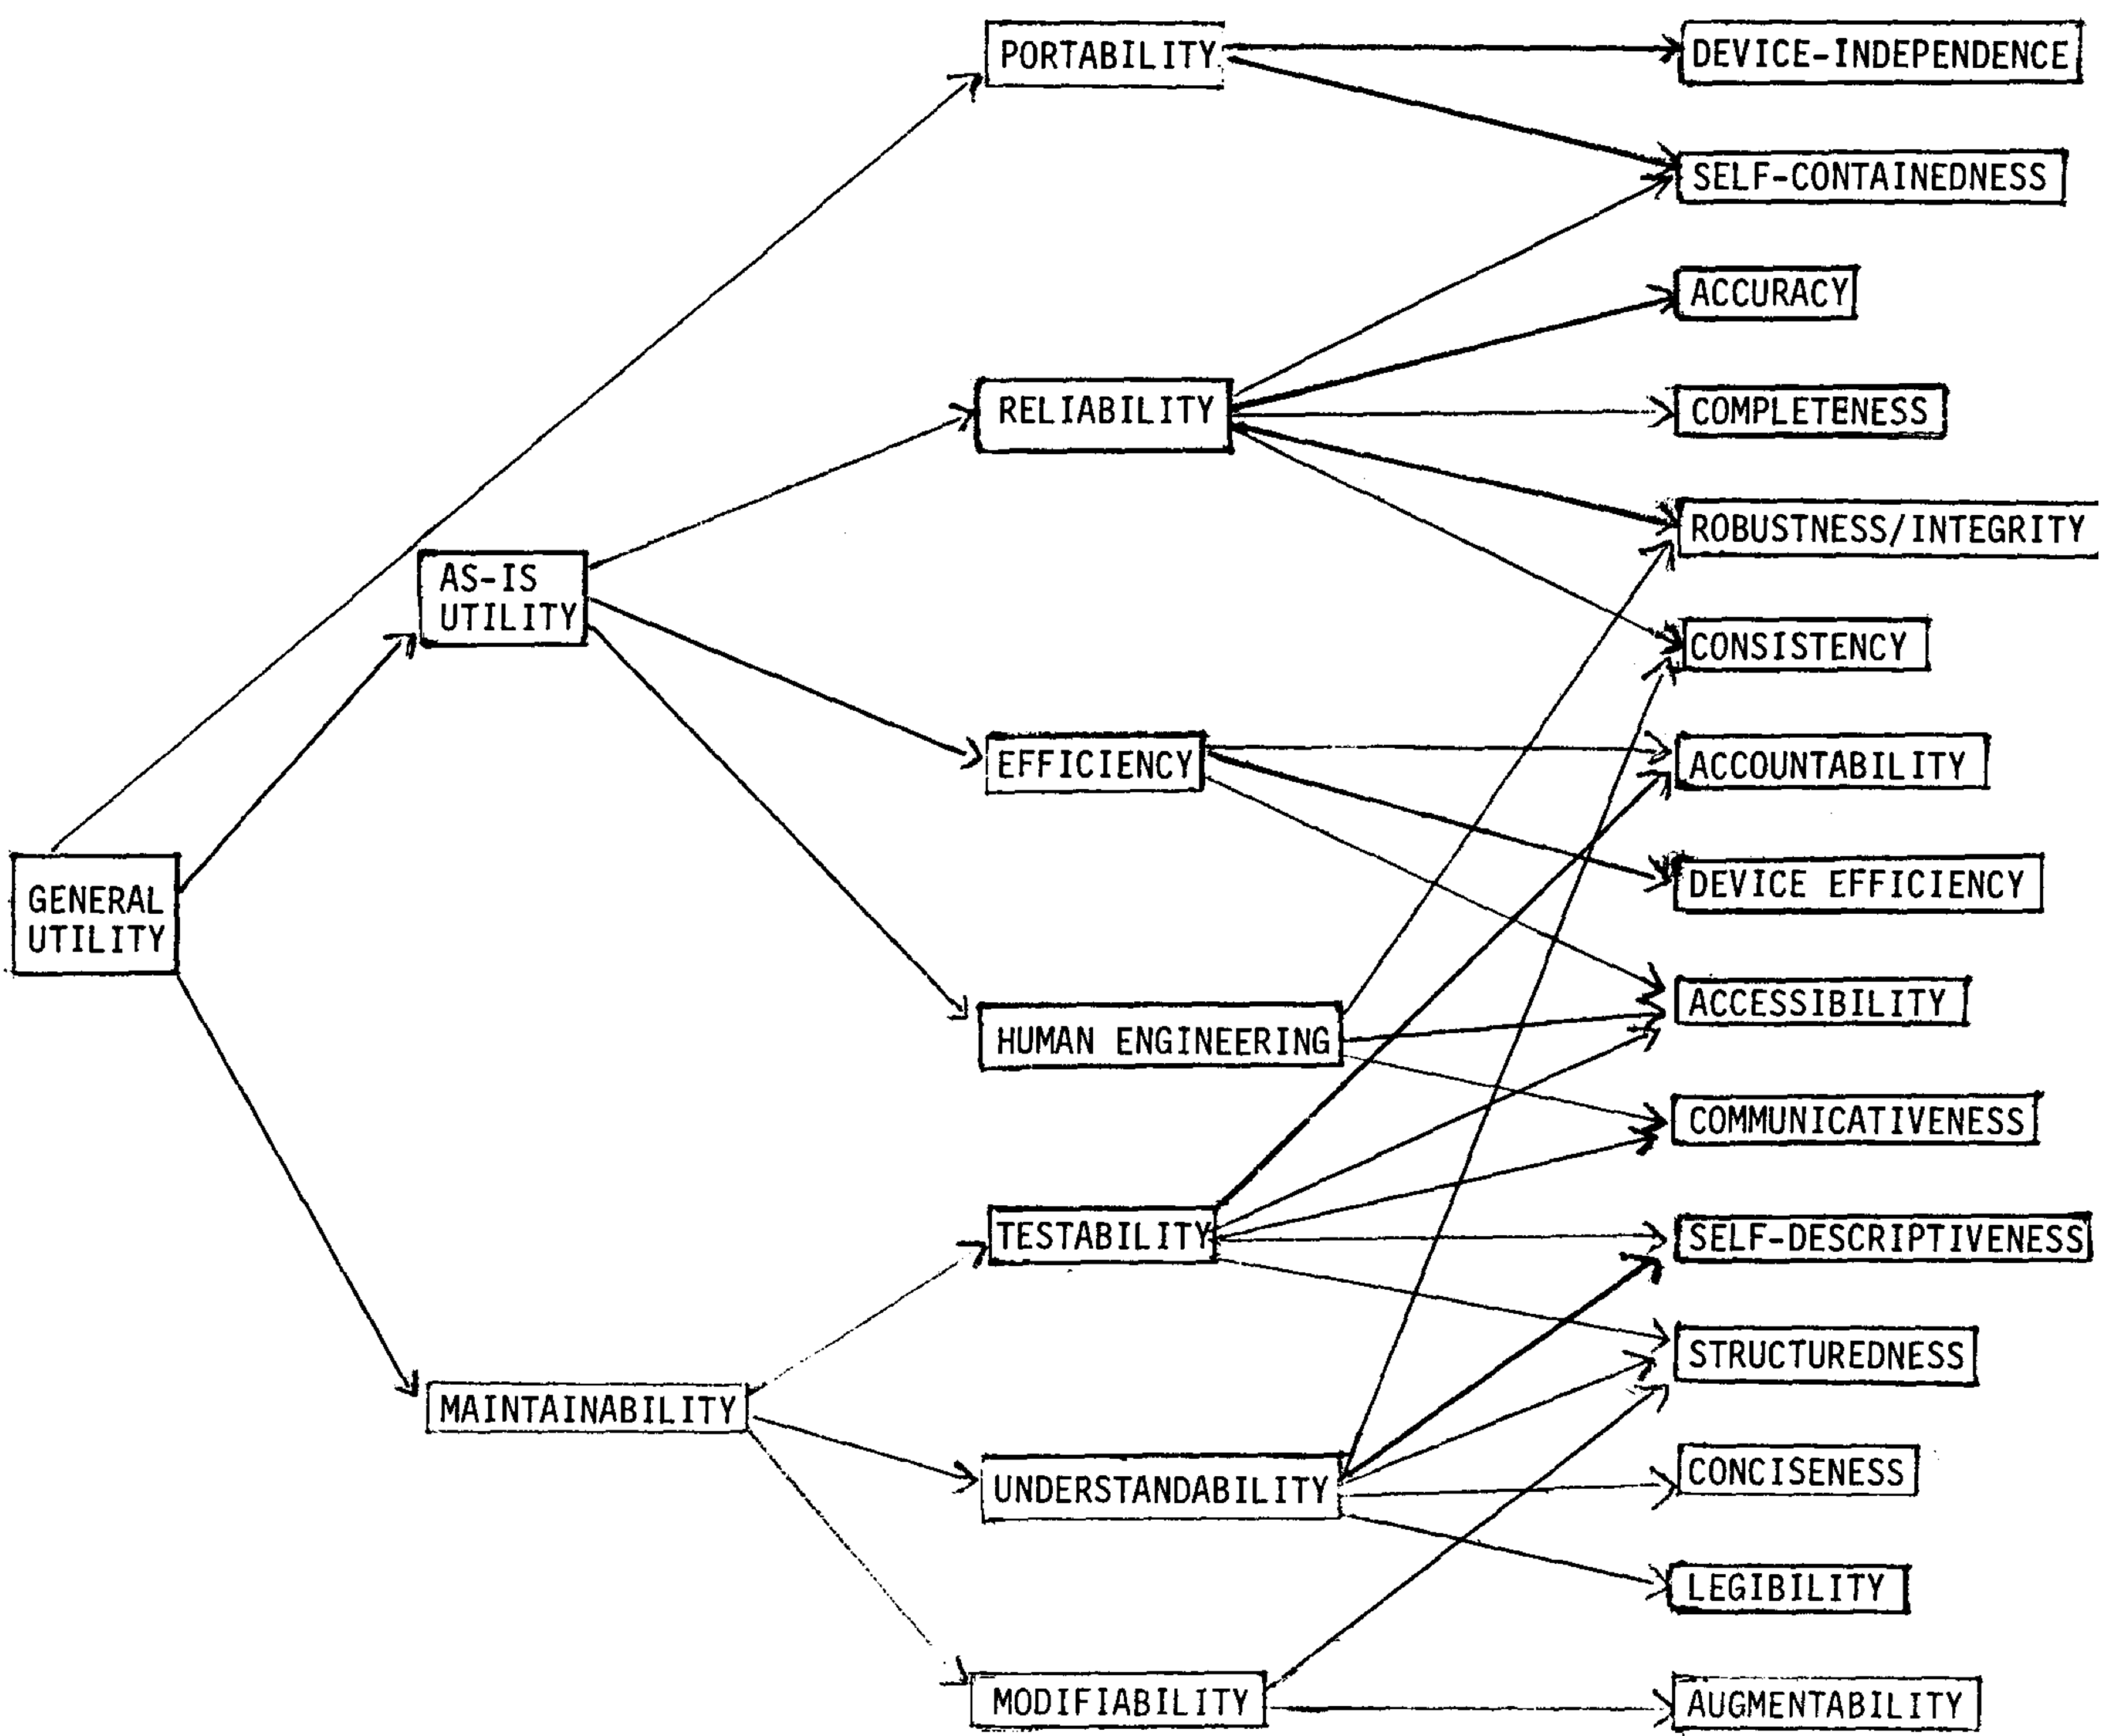
\includegraphics[width=0.8\linewidth]{bohems-software-quality-characteristics-tree}
    \caption{Bohem's Software Quality Characteristics Tree (\citeyear{Boehm:1978vv}) \citep{Boehm:1978vv}.}
    \label{fig:lit-review:software-quality:quality-models:development:boehm}
  \end{subfigure}
  ~
  \begin{subfigure}[t]{0.49\linewidth}
    \centering
    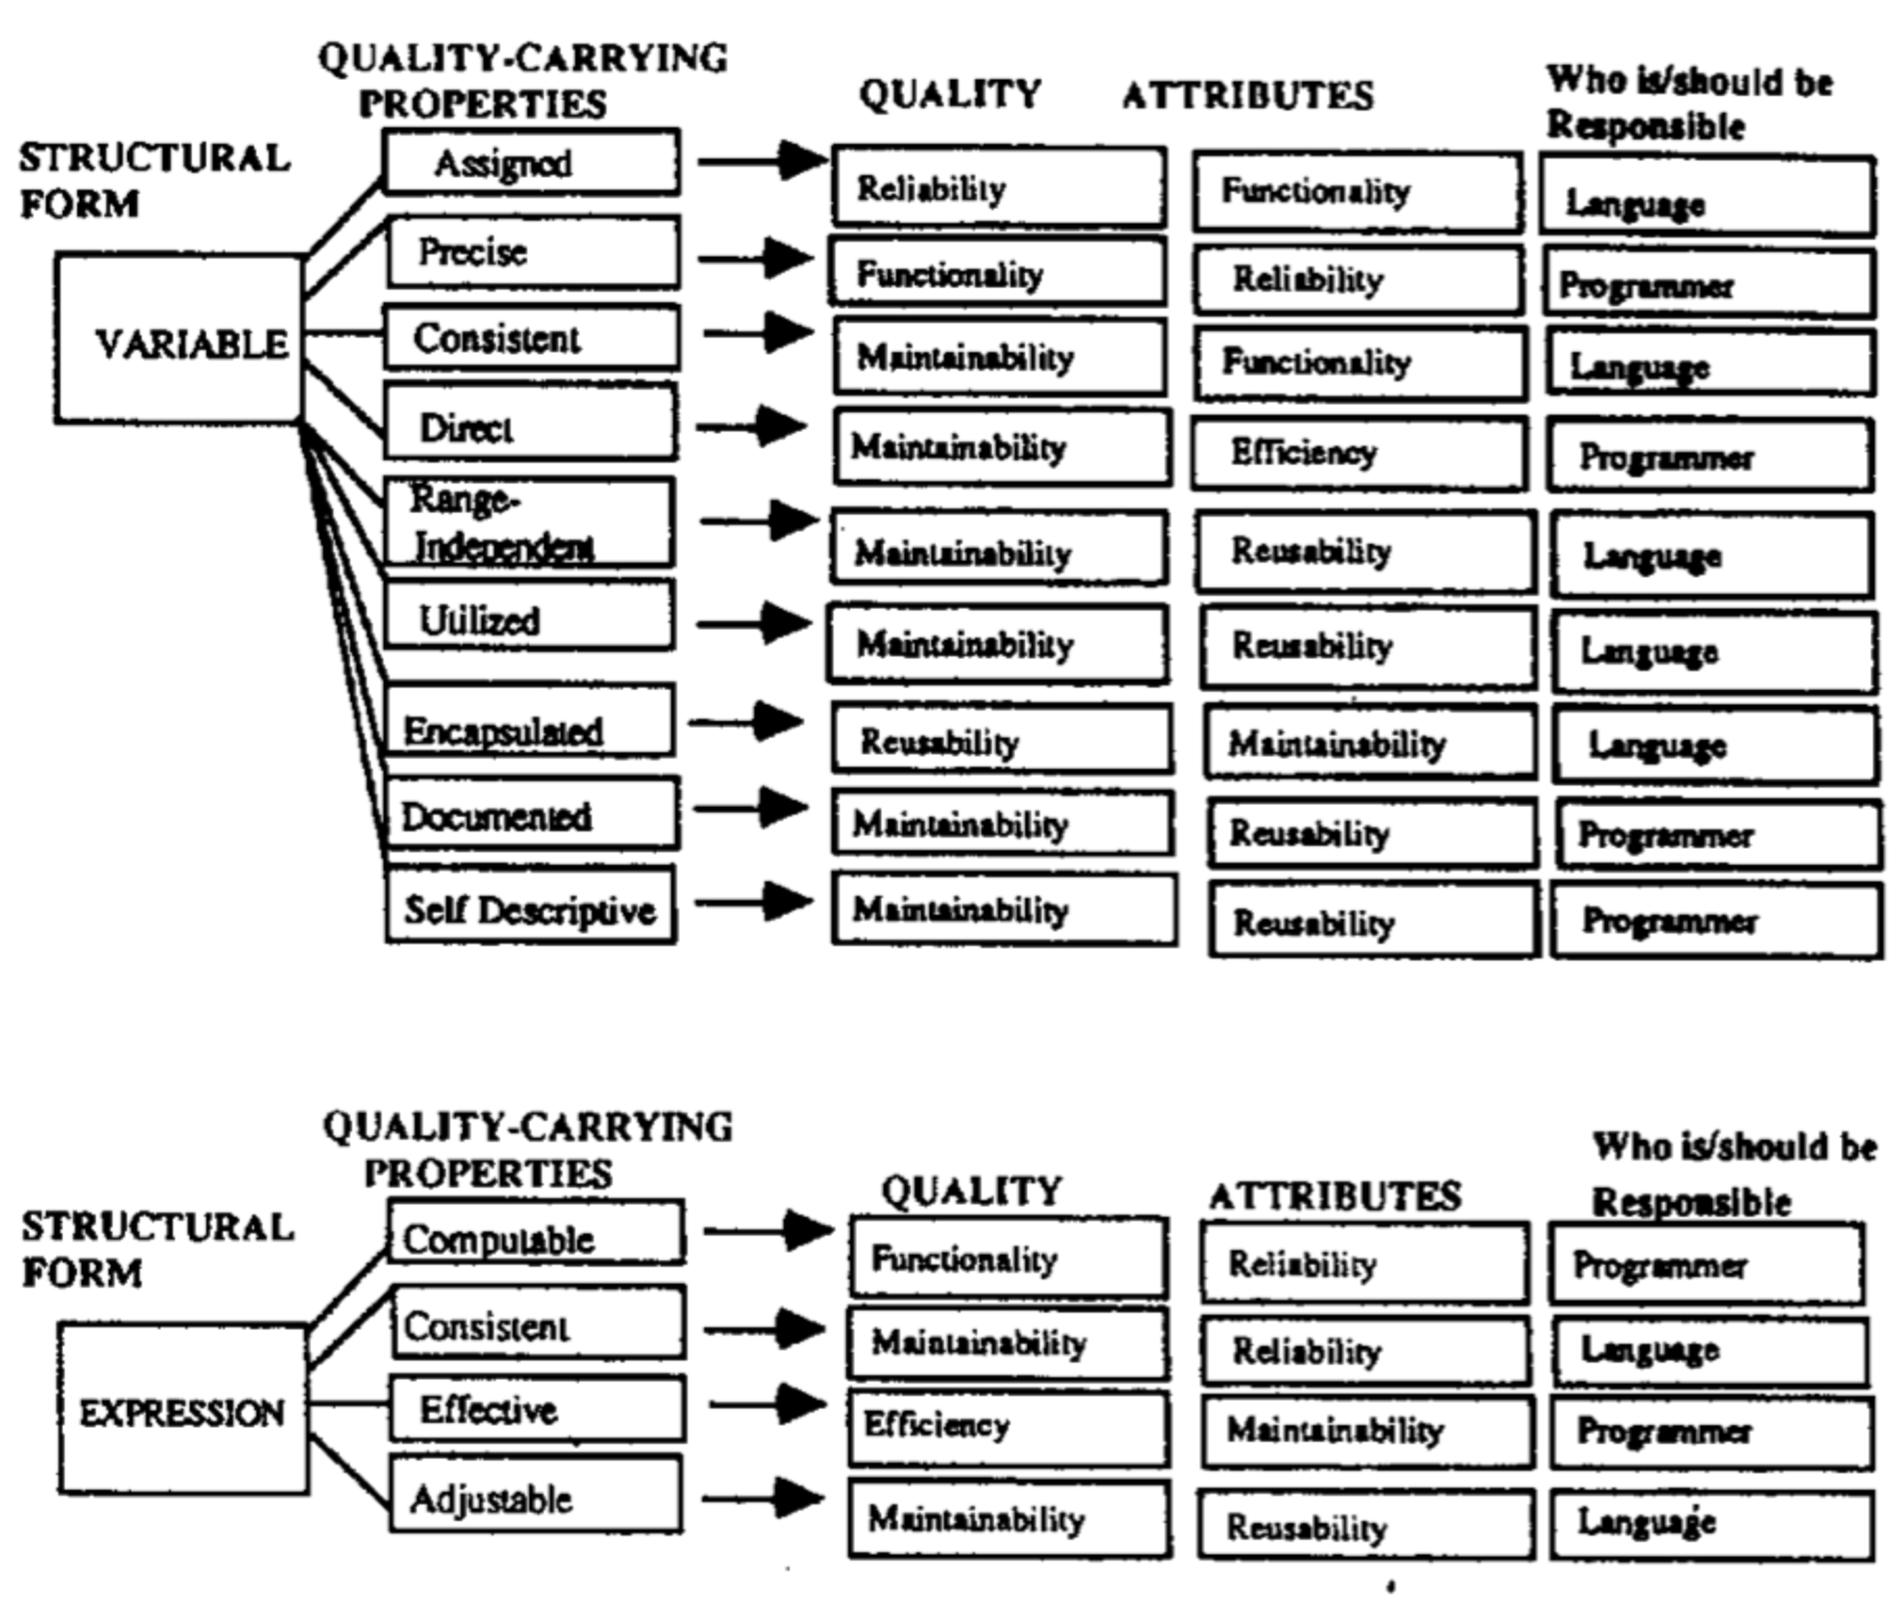
\includegraphics[width=0.8\linewidth]{dromey-quality-carrying-properites}
    \caption{Dromey's quality-carrying properties and programming languages (\citeyear{Dromey:1995wy}) \citep{Dromey:1995wy}.}
    \label{fig:lit-review:software-quality:quality-models:development:dromey}
  \end{subfigure}
  ~
  \begin{subfigure}[t]{0.49\linewidth}
    \centering
    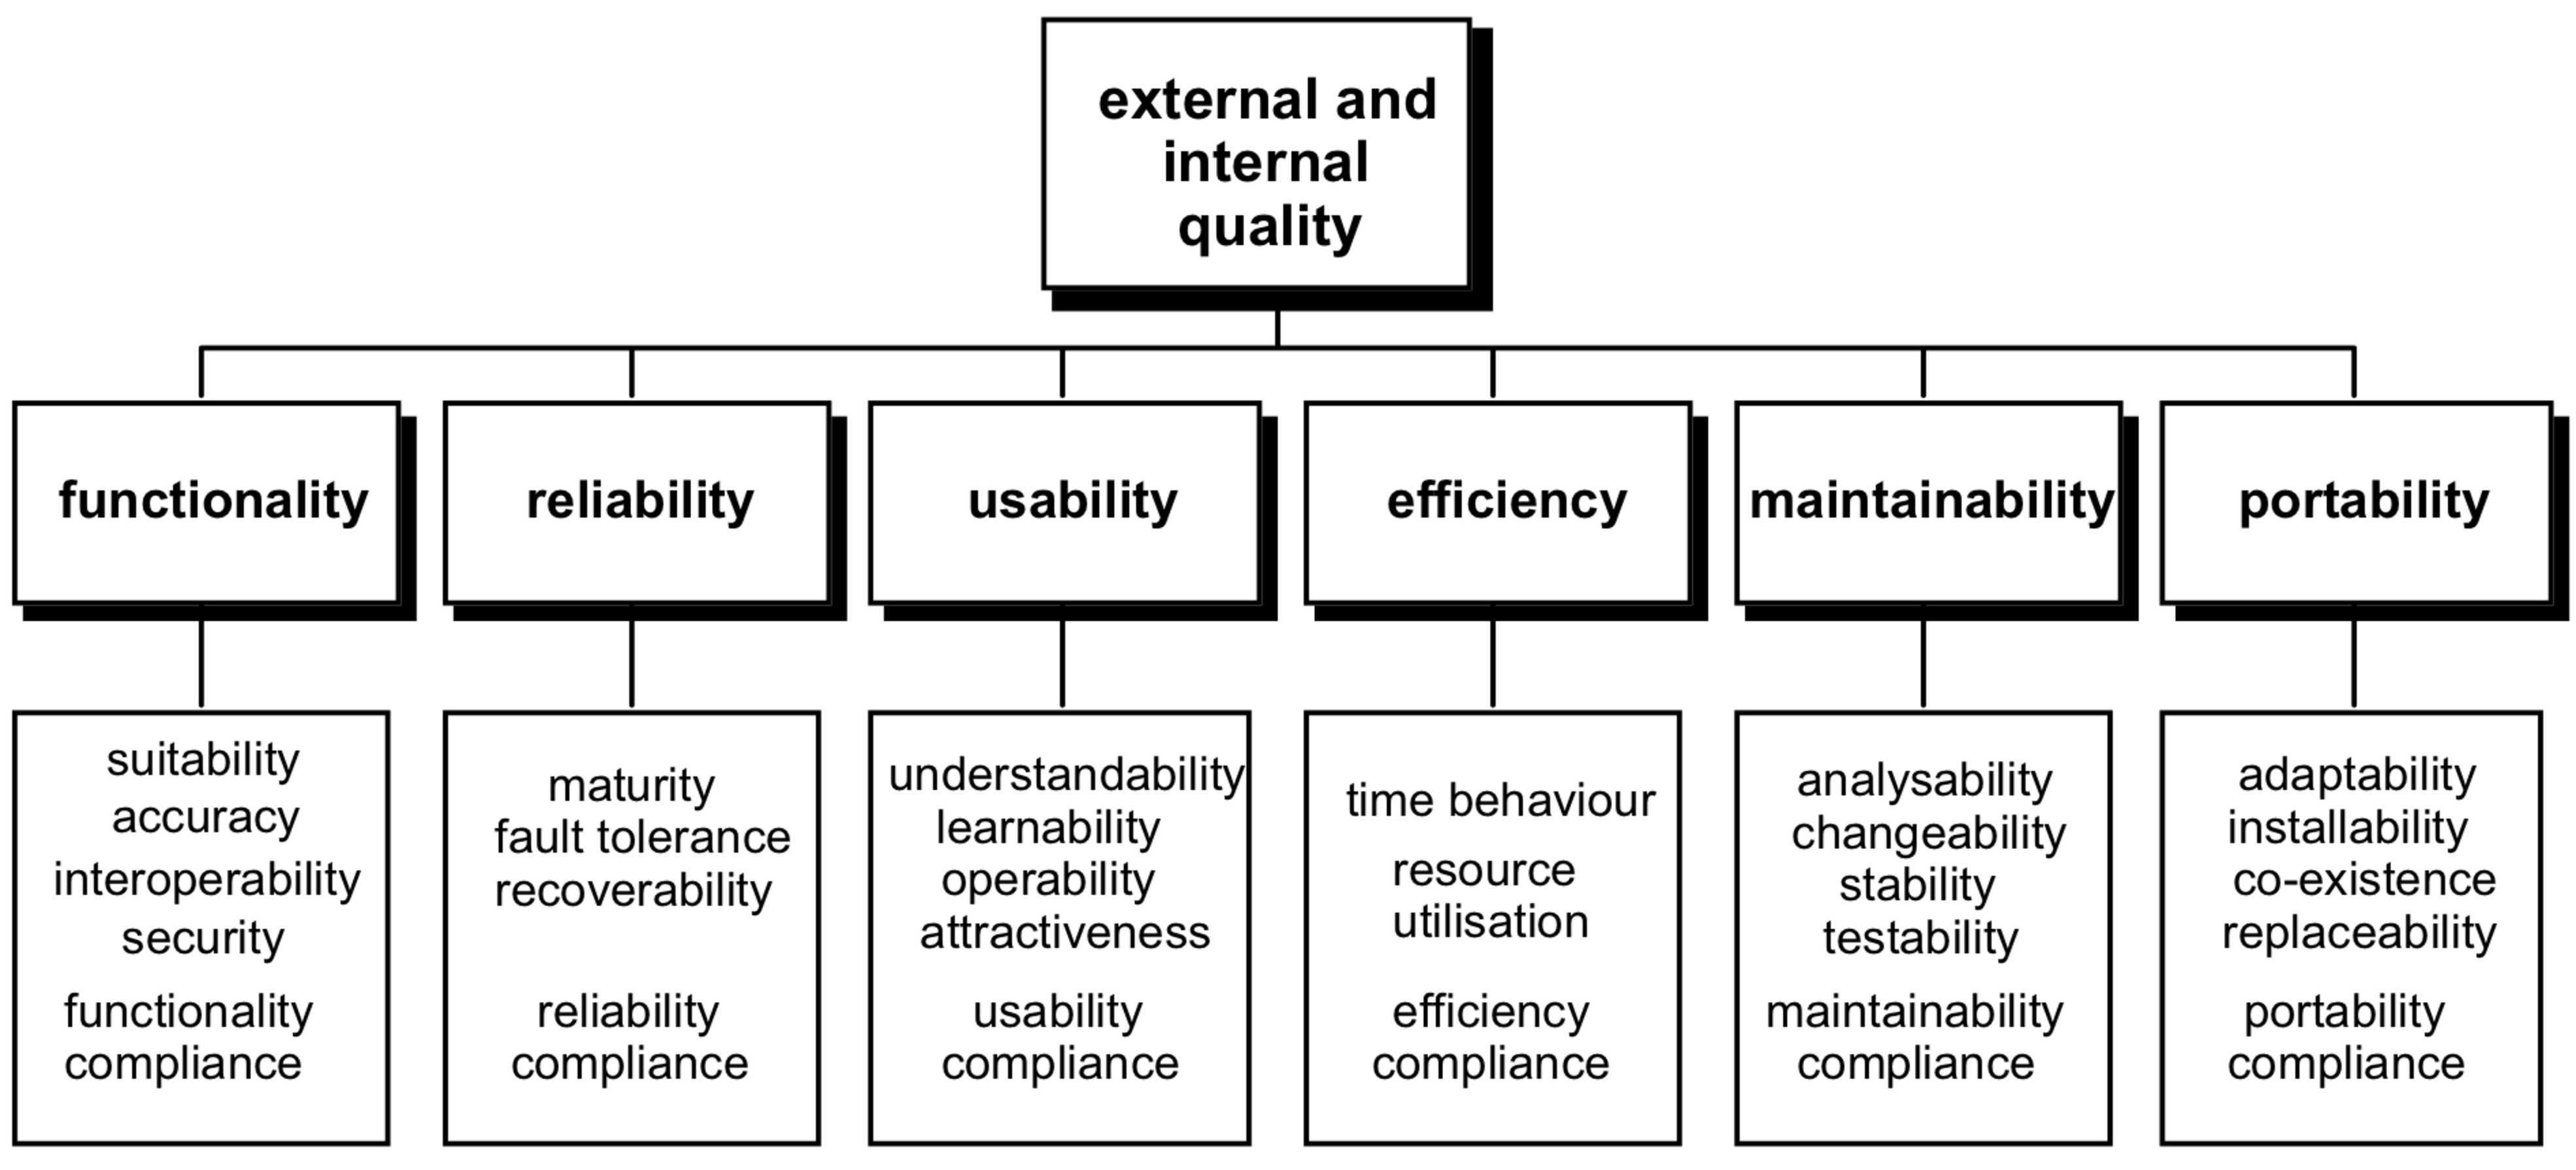
\includegraphics[width=\linewidth]{iso-software-product-evaluation-characteristics}
    \caption{ISO software product evaluation characteristics (\citeyear{ISO9126:1999}) \citep{ISO9126:1999}.}
    \label{fig:lit-review:software-quality:quality-models:development:iso}
  \end{subfigure}
  \caption{The brief overview of the development of software quality models since \citeyear{McCall:1977wm}.}
  \label{fig:lit-review:software-quality:quality-models:development}
\end{figure}

Of all the models described, there is one quality attribute that relates most with our narrative of \gls{cis} quality: reliability. The definition of reliability is largely the same among all quality models:

\begin{description}[font=\itshape,style=multiline,leftmargin=3cm]
  \item[\citeauthor{McCall:1977uy}] Extent to which a program can be expected to perform its intended function with required precision \citep{McCall:1977uy}.
  \item[\citeauthor{Boehm:1978vv}] Code possesses the characteristic \textit{reliability} to the extent that it can be expected to perform its intended functions satisfactorily \citep{Boehm:1978vv}.
  \item[\citeauthor{Dromey:1995bv}] Functionality implies reliability. The reliability of software is therefore largely dependent on the same properties as functionality, that is, the correctness properties of a program \citep{Dromey:1995bv}.
  \item[ISO-9126] The capability of the software product to maintain a specified level of performance when used under specified conditions \citep{ISO9126:1999}.
\end{description}

These definitions strongly relate to the solution description (\cref{ssec:lit-review:software-quality:solution-description}) in that reliability is the ability to maintain functionality under given conditions. But what defines reliability when the nature of a \gls{cis} in itself is inherently unpredictable due to its probabilistic implementation? Can a non-deterministic system ever be considered reliable when the output of the system is uncertain? How do developers perceive these quality aspects of reliability in the context of such systems? Therefore, we believe the literature of quality models does not suffice in the context of \gls{cis} reliability; a computer vision \gls{cis} can interpret an image of a dog as a `Dog' one day, but what if the next it interprets such image more specifically to the breed, such as `Border Collie'? Does this now mean the system is unreliable? 

Moreover, defining these systems in themselves is challenging when requirements specifications and solution descriptions are totally dependent on probabilistic outcomes. We explore this concept in further detail within the following subsection.

\subsection{Solution Description}
\label{ssec:lit-review:software-quality:solution-description}